%\documentclass[aspectratio=43]{beamer}
%\documentclass[aspectratio=169]{beamer}
\documentclass[aspectratio=1610,12pt]{beamer}
\usepackage[utf8]{inputenc}
\usepackage[T1]{fontenc}
\usepackage{lmodern}

\usepackage[ngerman]{babel}
%\usepackage[ngerman]{babel} %use this for German presentations
\usepackage{booktabs} % fancy tables
\usepackage{tabulary} % tables with auto column length
\usepackage{hyperref}

\usetheme{imise2}
\author{Maryam Ghalandari \& Konrad Höffner \& Thomas Pause}
\date{Leipzig, 15.Mai 2020}
\title{Instance Generator}
\subtitle{How to model and software products with}
\def\address{Härtelstraße 16-18, 04107 Leipzig, Raum 227}
\def\email{maryam.ghalandari@imise.uni-leipzig.de}
\def\telephone{~}

\usepackage{setspace}

\begin{document}
\begin{frame}
\titlepage
\end{frame}

\begin{frame}{Überblick}
\begin{spacing}{1.25}
\begin{enumerate}
\item Die HITO Ontologie
\item Instance Generator
~\\ ~\\
\item Catalogues and citations
\item Examples
\end{enumerate}
\end{spacing}
\end{frame}

\begin{frame}{Das O in HITO -- Die Ontologie}
\centering
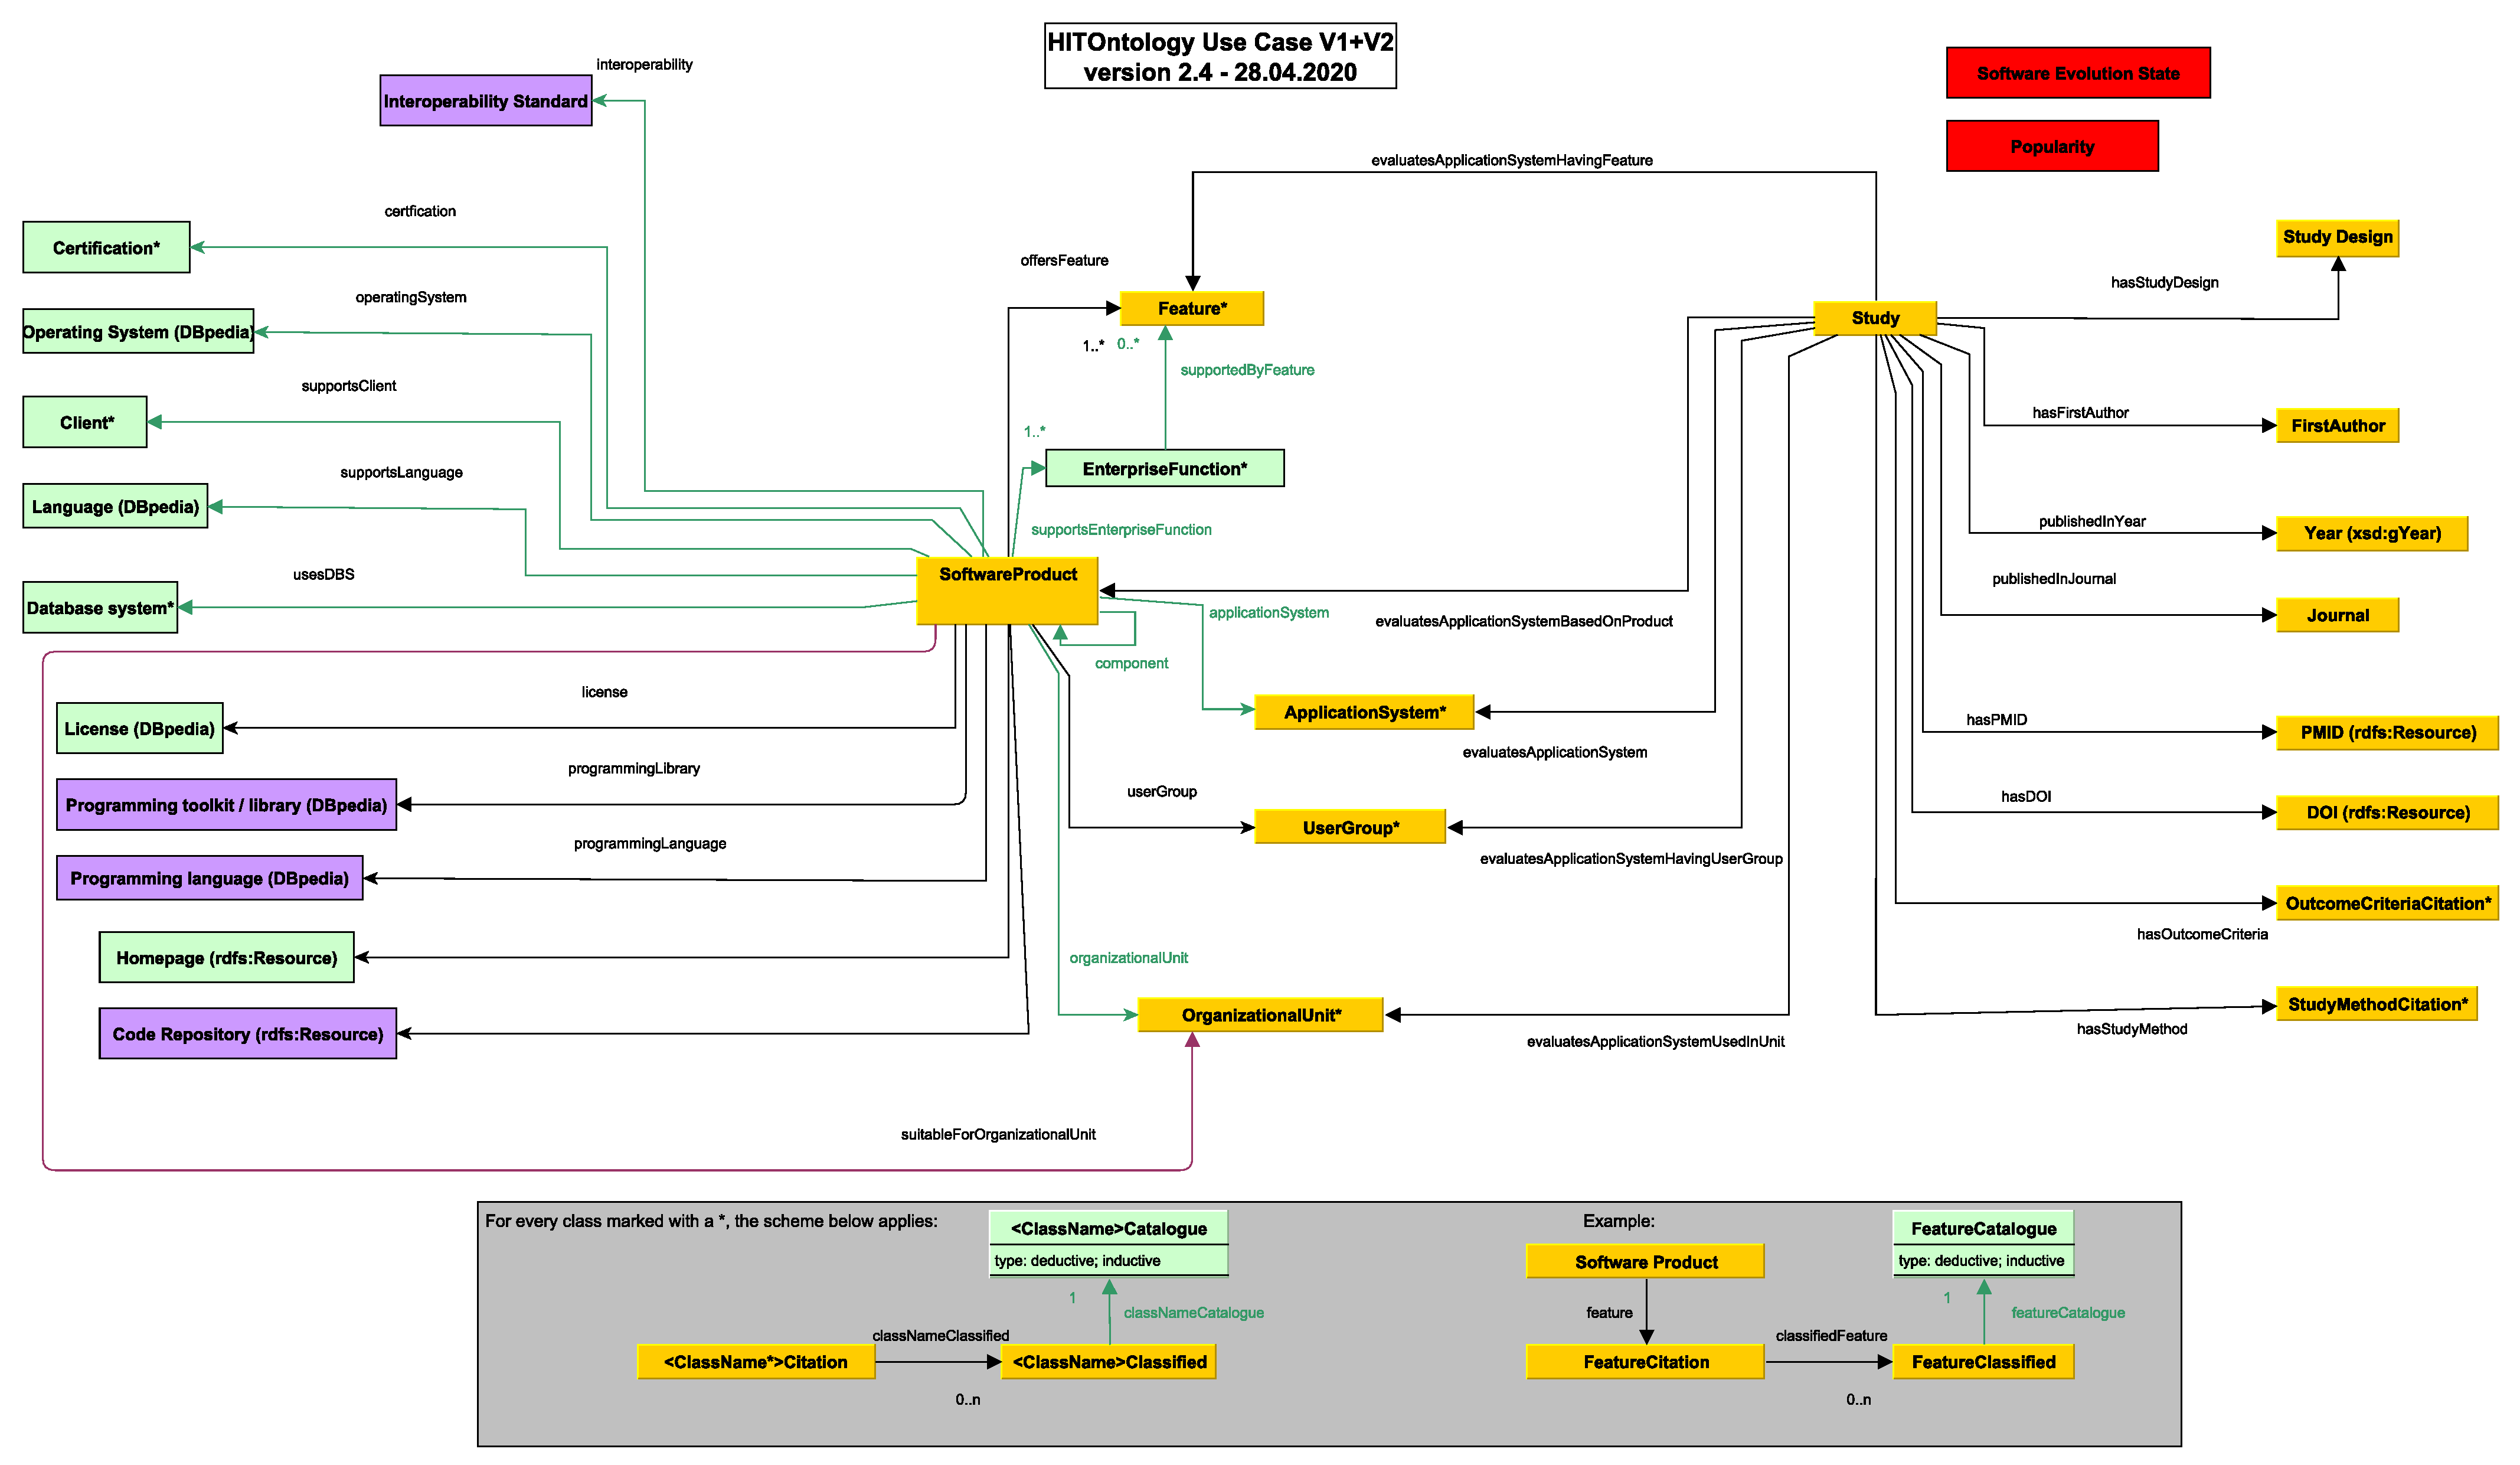
\includegraphics[width=.95\textwidth]{img/HITontology.pdf}
\end{frame}

\begin{frame}{Software Products in HITO}
\centering
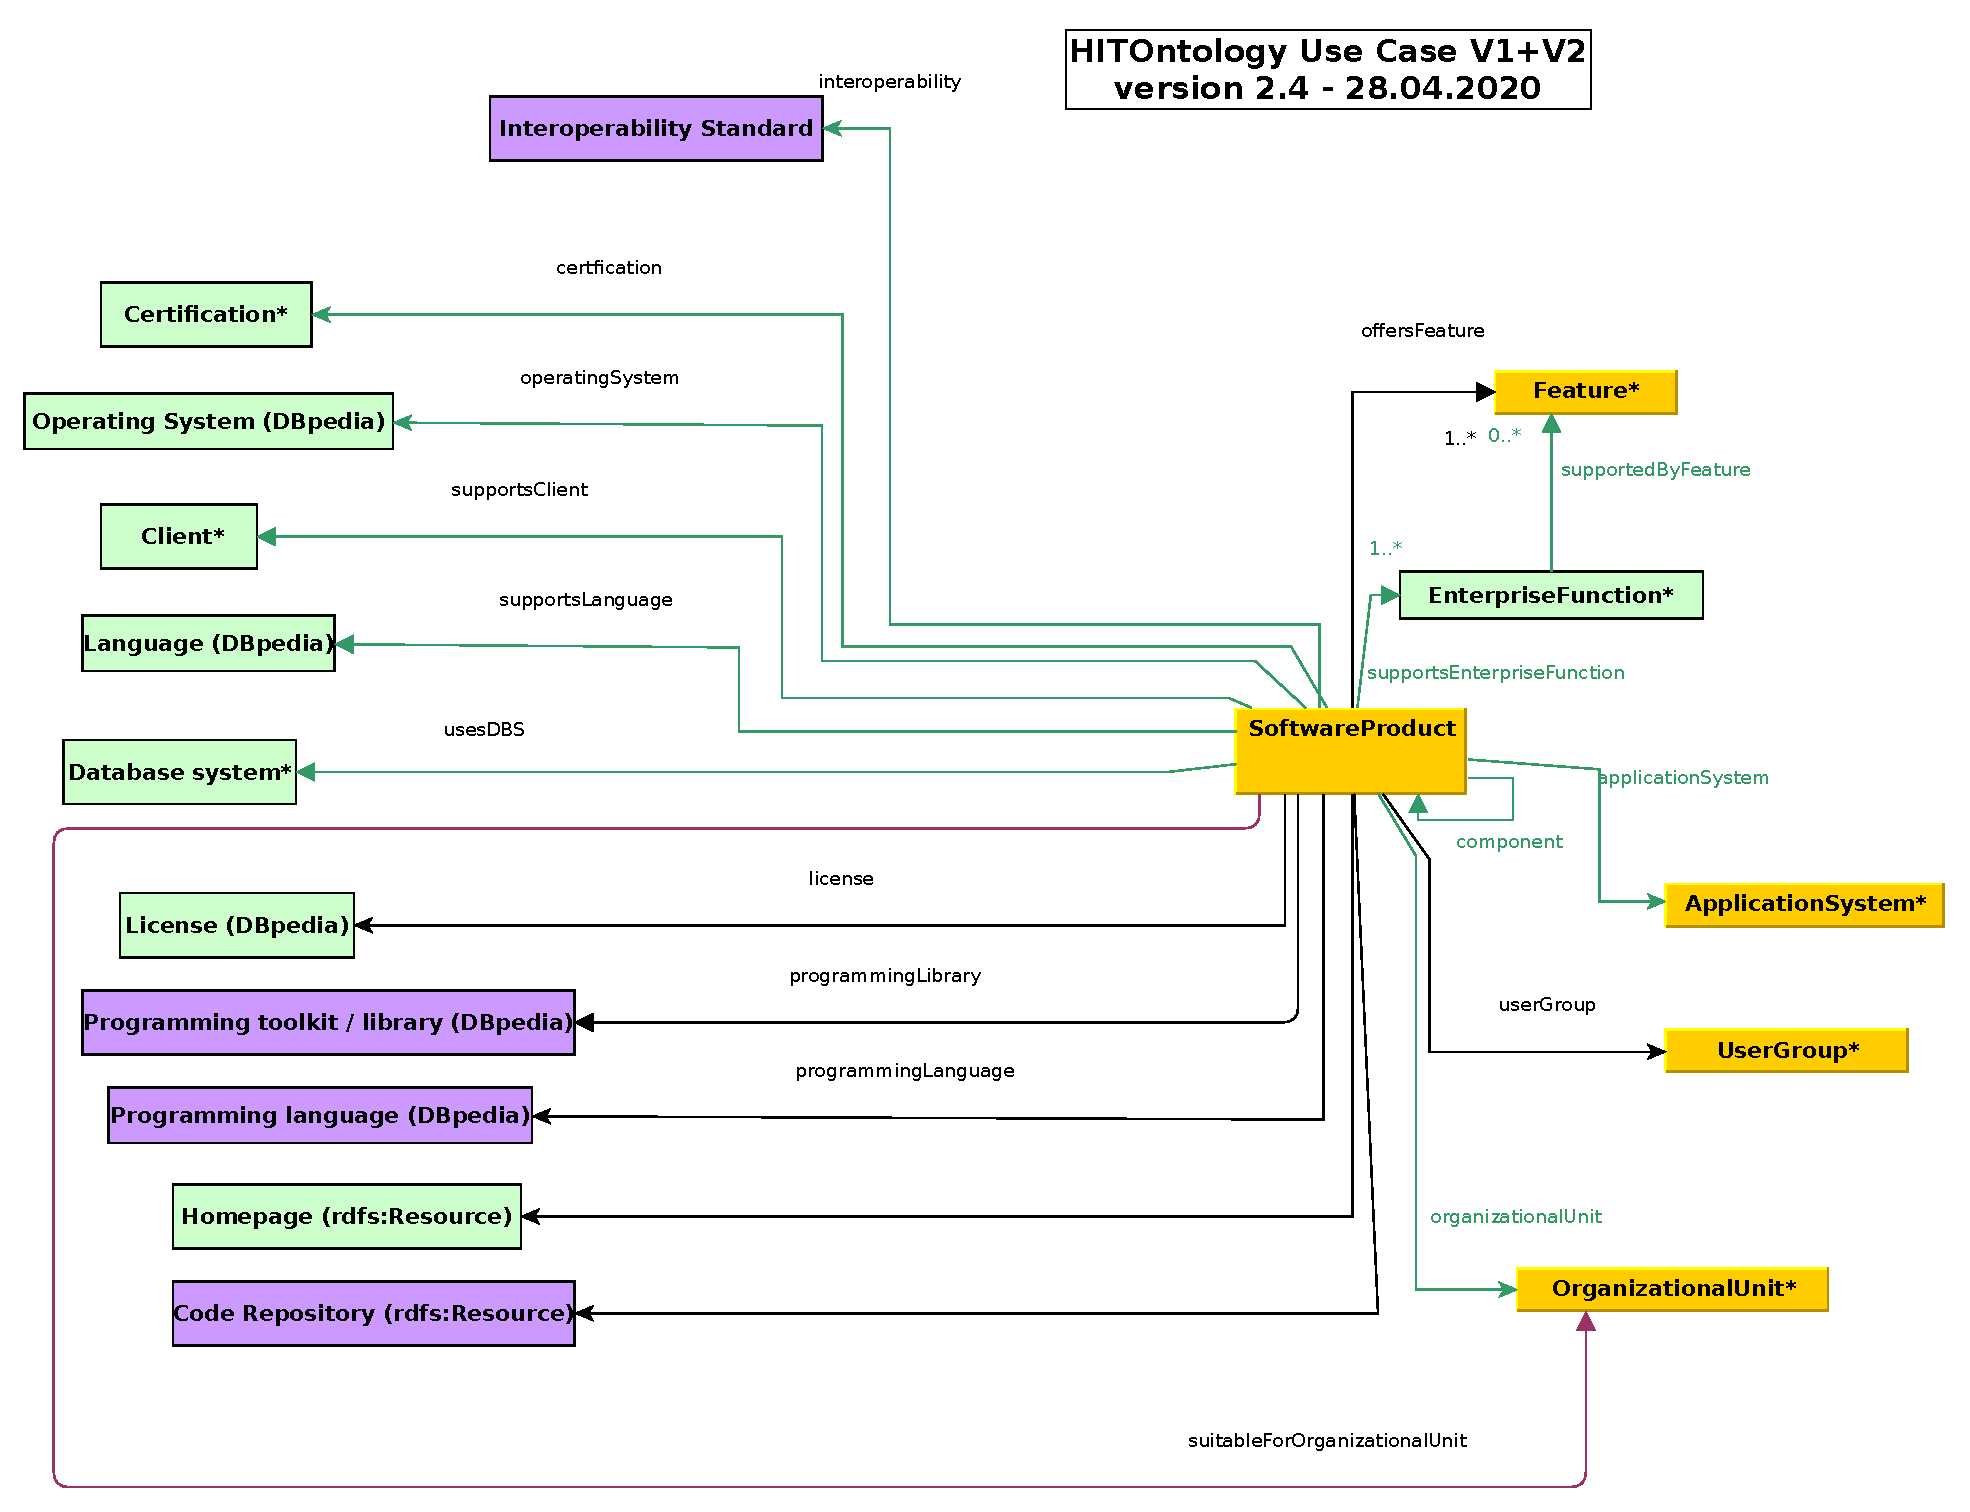
\includegraphics[height=.8\textheight]{img/excerpt2.pdf}
\end{frame}

\begin{frame}{HITO Linked Data Lifecycle}
  \centering
  \vspace{-0.5cm}
  \includegraphics[height=0.85\textheight]{hitocyclestart.pdf}
\end{frame}

\begin{frame}{HITO Lifecycle Model}
  \centering
  \vspace{-0.5cm}
  \includegraphics[height=0.85\textheight]{hitocyclemodel.pdf}
\end{frame}

\begin{frame}{Instance Generator}
\begin{spacing}{1.25}
\begin{itemize}
\item verfügbar als GitHub Page unter:
\begin{itemize}
\item \url{https://hitontology.github.io/instancegenerator/}
\end{itemize}
\item Werkzeug zum Erzeugen neuer Instanzen der Ontologie
\item Produkte werden mit zahlreichen Attributen modelliert
\item Nutzung von individuellen Katalogen
\item Video-Demonstration:
\begin{itemize}
\item \url{https://youtu.be/EWvEaSCo3Vg}
\end{itemize}
\end{itemize}
\end{spacing}
\end{frame}

% \begin{frame}{Maryams part}
% from now on Maryam is speaking
% \end{frame}

\begin{frame}{Catalogues and citations}
\pause
\centering
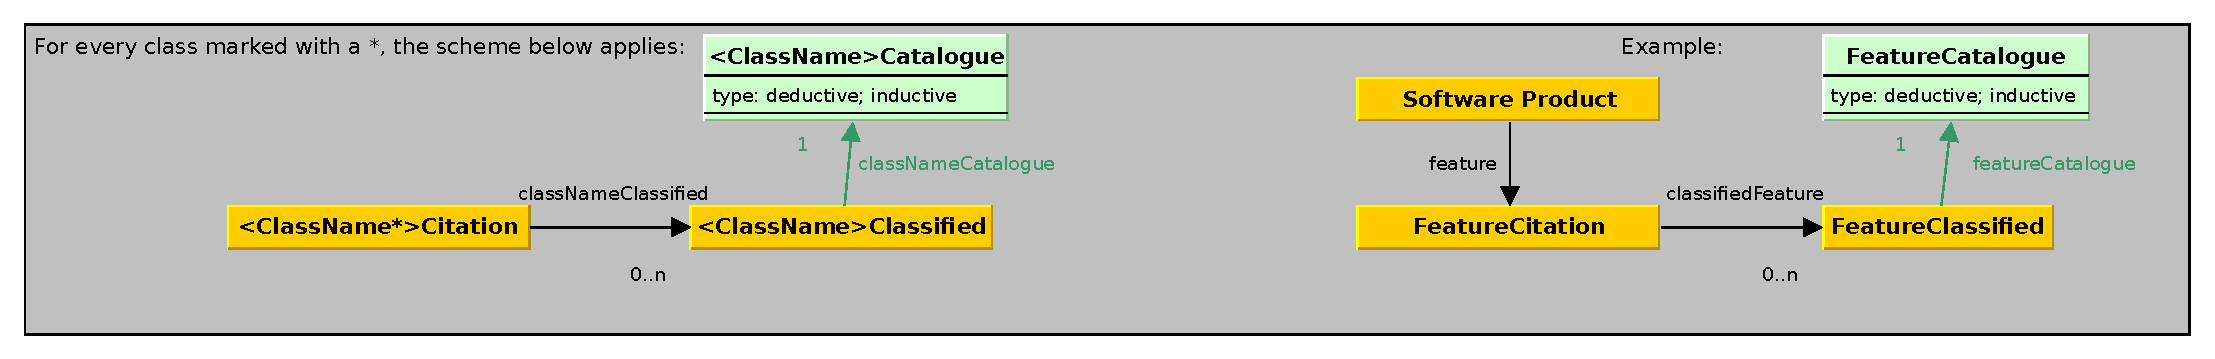
\includegraphics[width=\textwidth]{img/excerpt1.pdf}
\end{frame}

\begin{frame}{Catalogues and citations}
\begin{columns}
  \column{0.35\linewidth}
  \vspace{-1cm}
  \begin{spacing}{1.25}
    \begin{itemize}
      \item our five catalogue types
      \begin{itemize}
        \item Application System
        \item Enterprise Function
        \item Feature
        \item User Group
        \item Organizational Unit
      \end{itemize}
    \end{itemize}
  \end{spacing}
  \column{.6\linewidth}
  \centering
  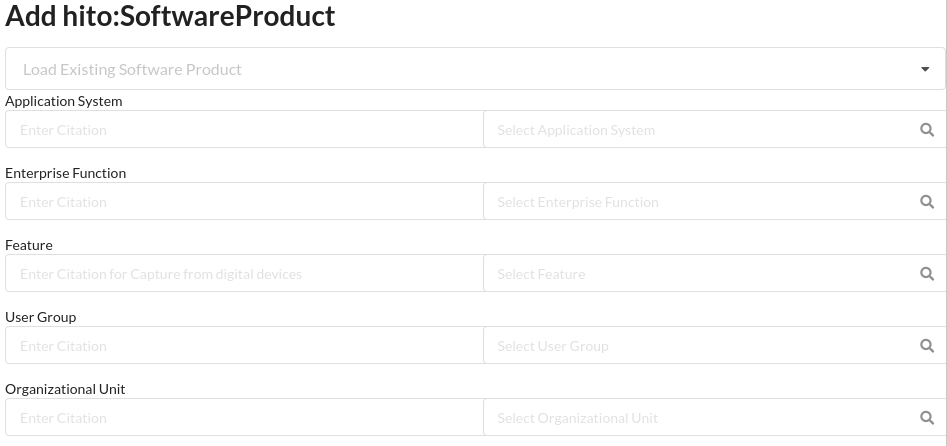
\includegraphics[width=\textwidth]{img/iglook.png}
\end{columns}
\end{frame}

\begin{frame}{HITO Lifecycle Browse}
  \centering
  \vspace{-0.5cm}
  \includegraphics[height=0.85\textheight]{hitocyclebrowse.pdf}
\end{frame}

\begin{frame}{Software Products in HITO Ontology (with LODView)}
\centering
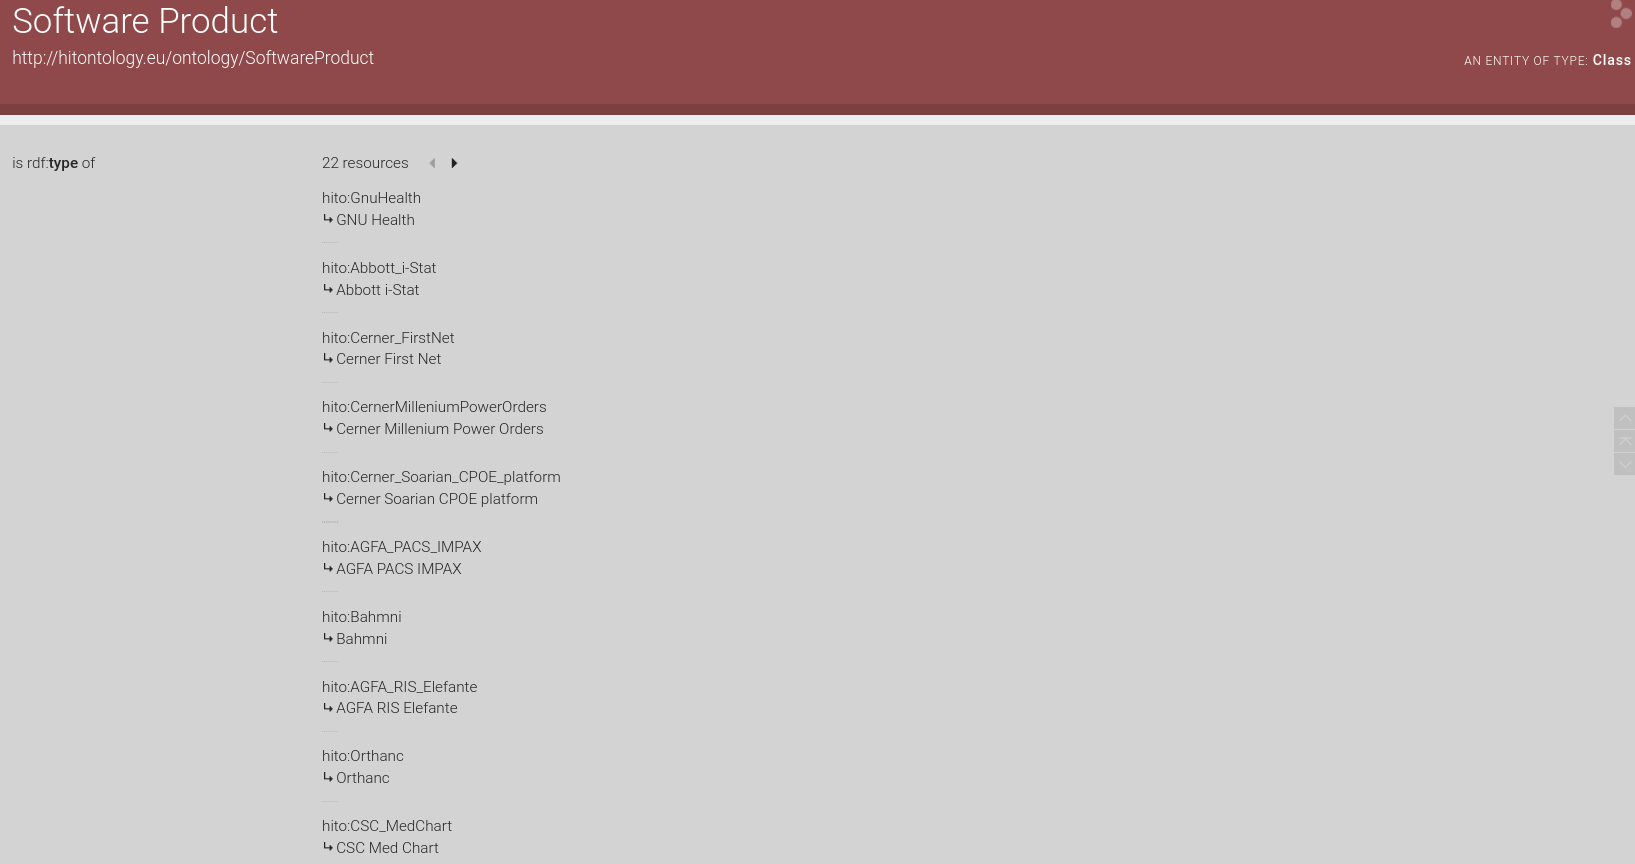
\includegraphics[width=\textwidth]{img/softwareproduct.png}
\end{frame}


\begin{frame}{Example I: GNU Health in LODView}
\vspace{-0.3cm}
\centering
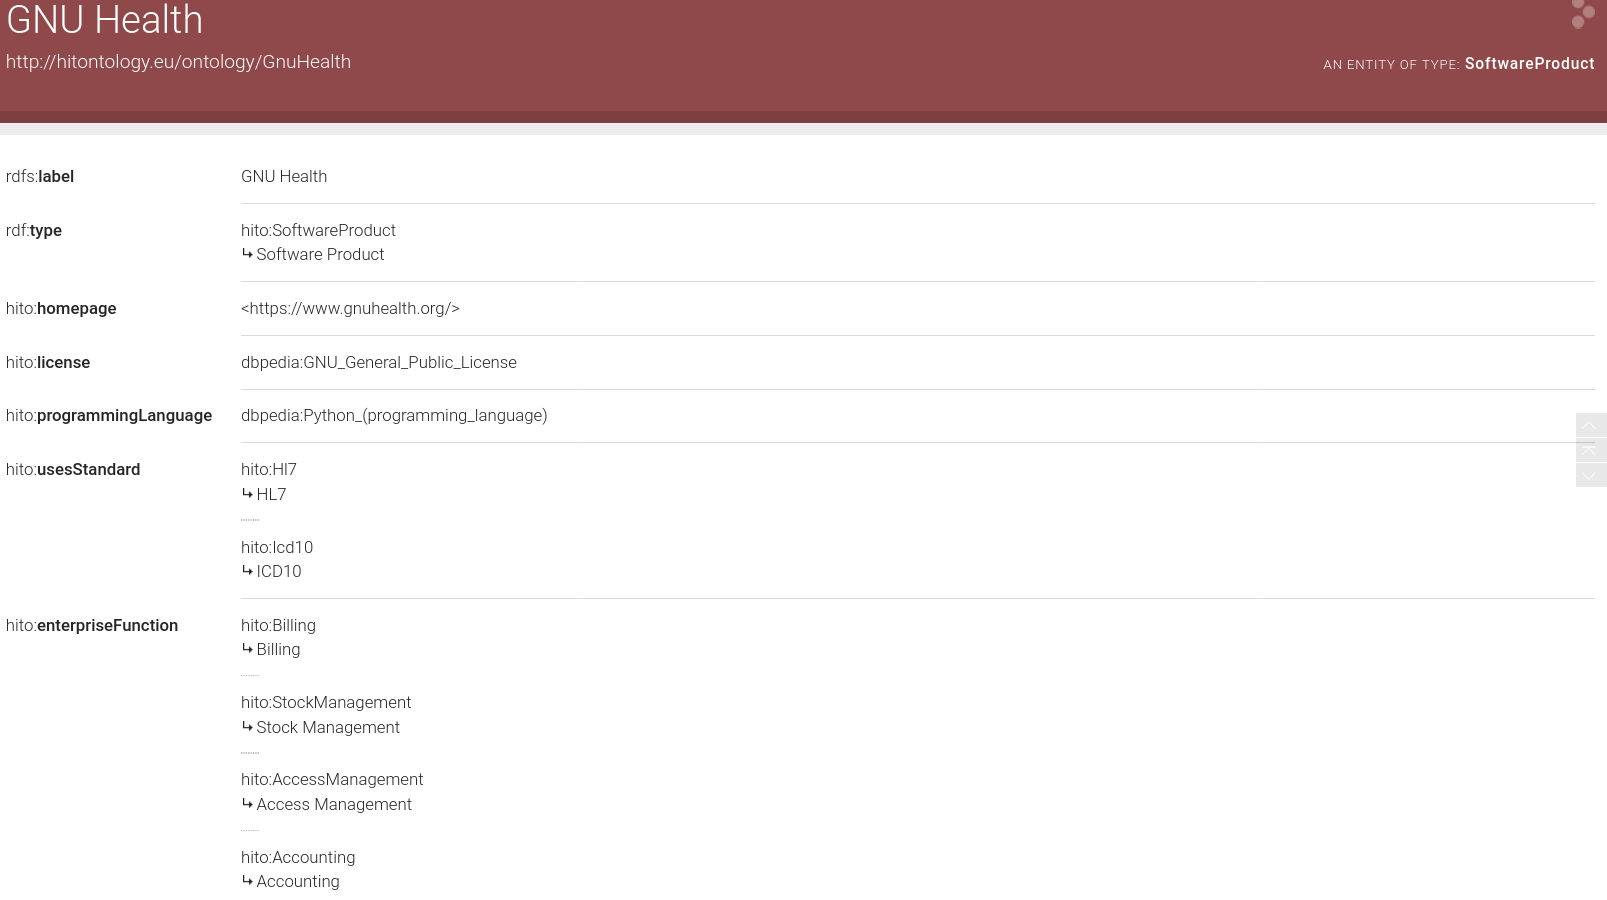
\includegraphics[width=.95\textwidth]{img/GnuHealth.png}
\footnotesize{\url{https://hitontology.eu/ontology/GnuHealth}}
\end{frame}

\begin{frame}{Example II: Bahmni in LODView}
\vspace{-0.3cm}
\centering
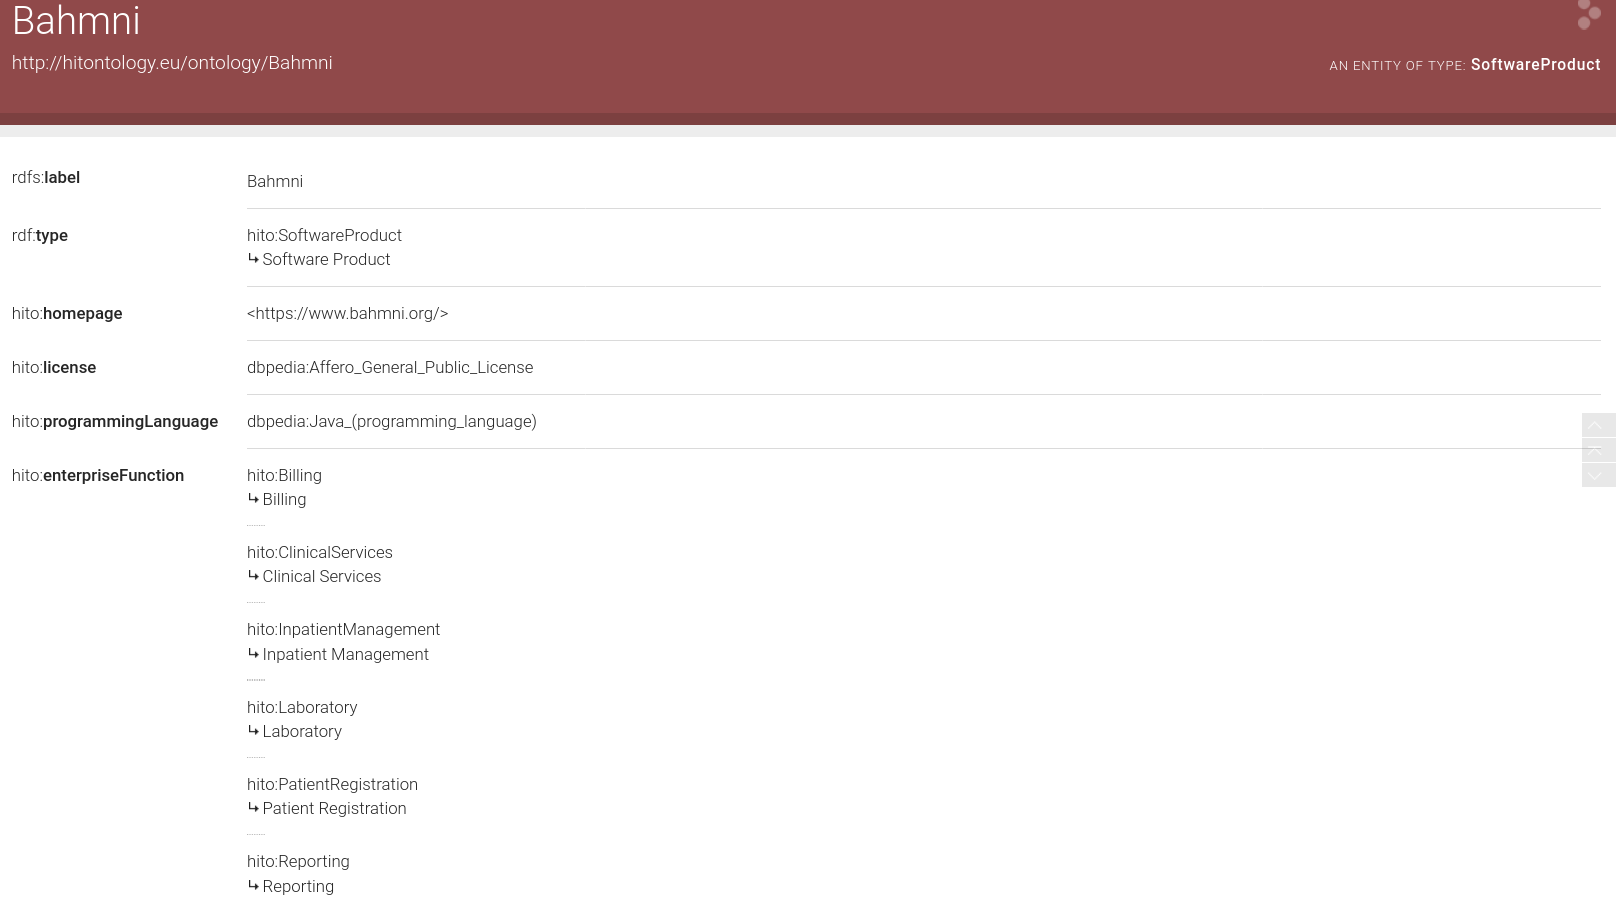
\includegraphics[width=.95\textwidth]{img/bahmni.png}
\footnotesize{\url{https://hitontology.eu/ontology/Bahmni}}
\end{frame}

\begin{frame}{Example II: Bahmni as graph (excerpt)}
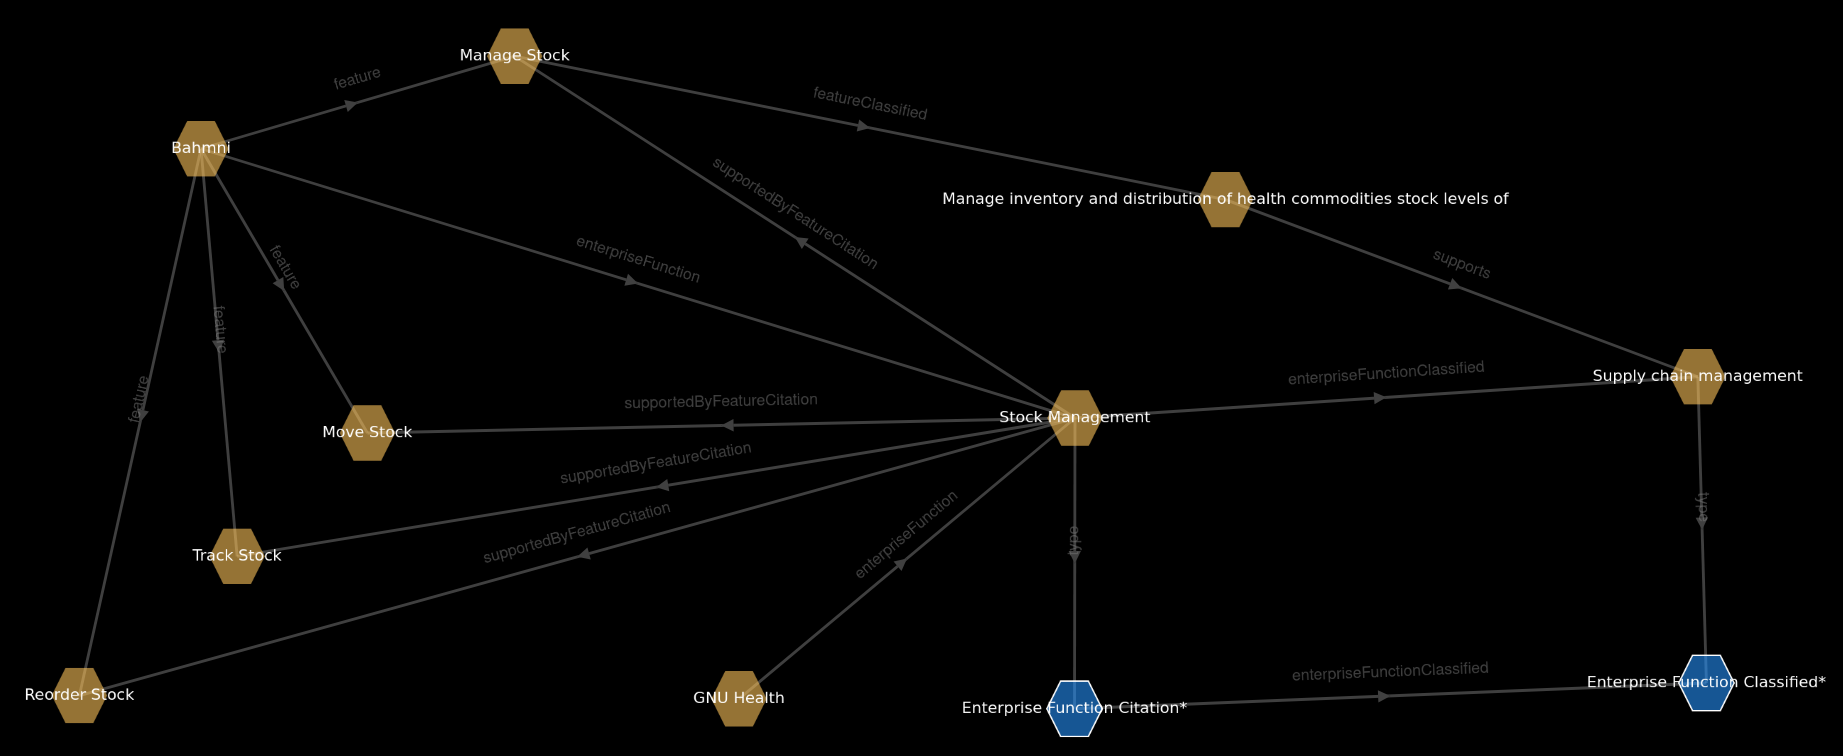
\includegraphics[width=\textwidth, height=.65\textheight]{img/bahmni_star.png}
\end{frame}

\begin{frame}{Catalogue connection of Supply Chain Management}
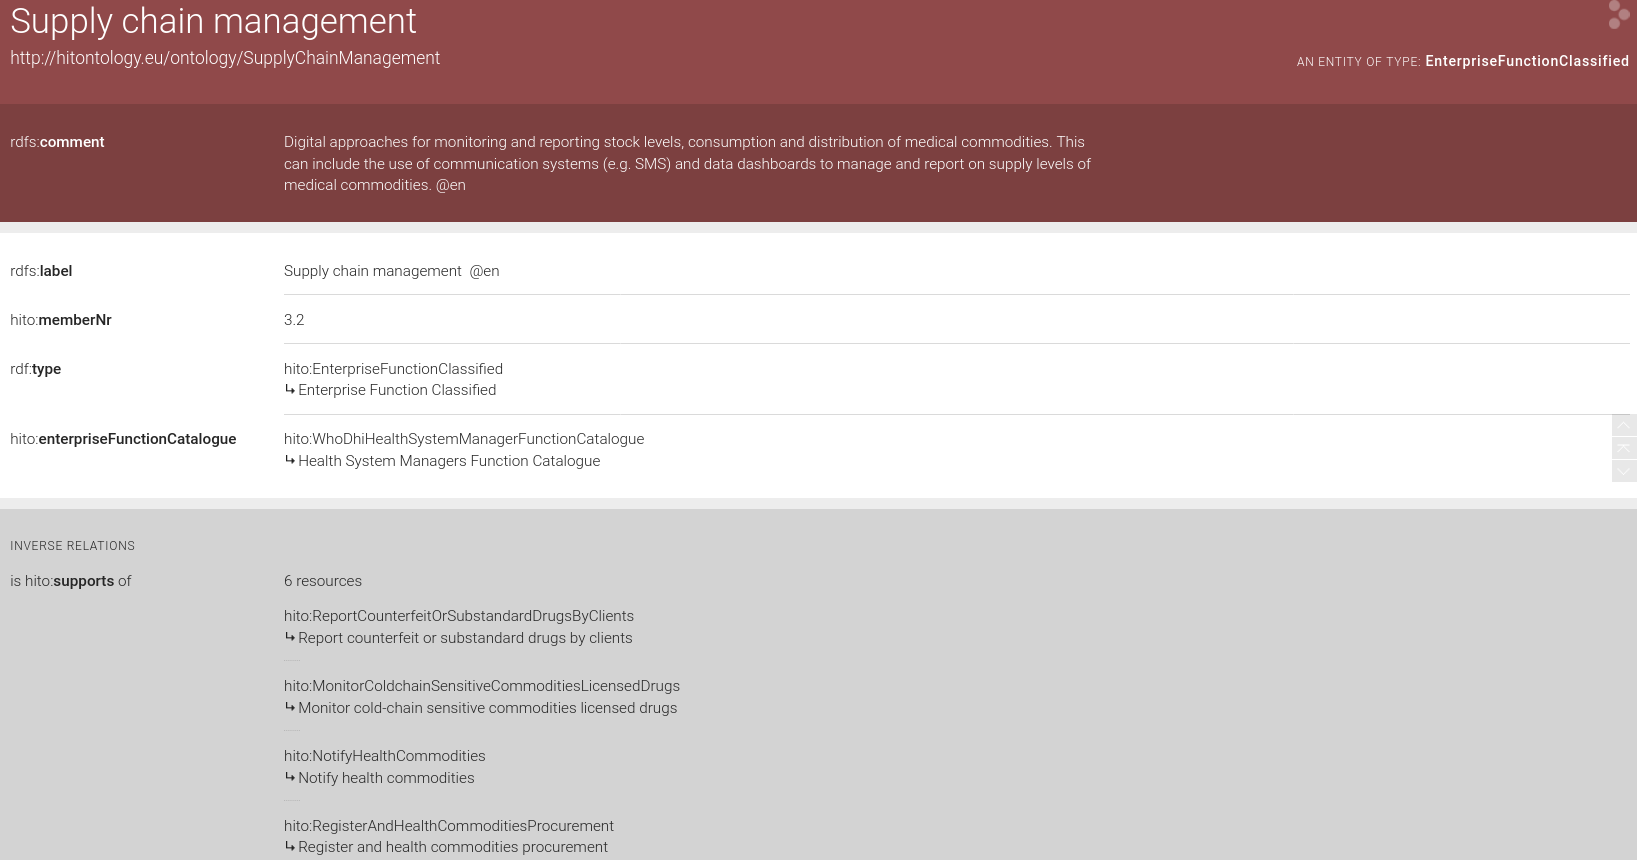
\includegraphics[width=\textwidth]{img/supplychainmanagement.png}
\end{frame}

\begin{frame}{HITO Lifecycle Search/Explore}
  \centering
  \vspace{-0.5cm}
  \includegraphics[height=0.85\textheight]{hitocyclesearch.pdf}
\end{frame}


\begin{frame}{Hito Bahmni}
  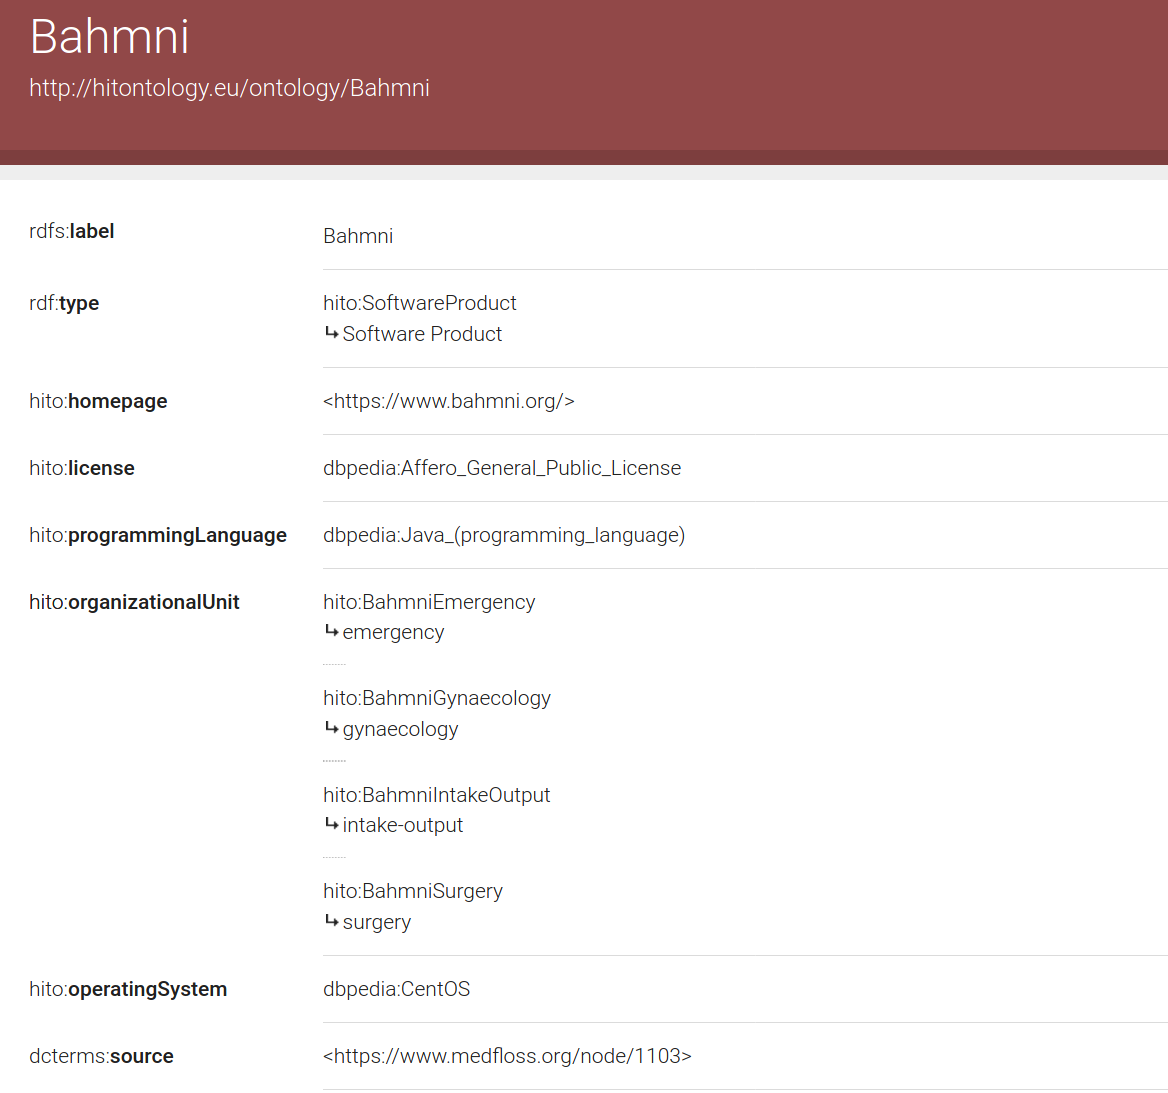
\includegraphics[width=\textwidth]{img/hito-bahmni.png}
\end{frame}

\begin{frame}{Medfloss Bahmni}
  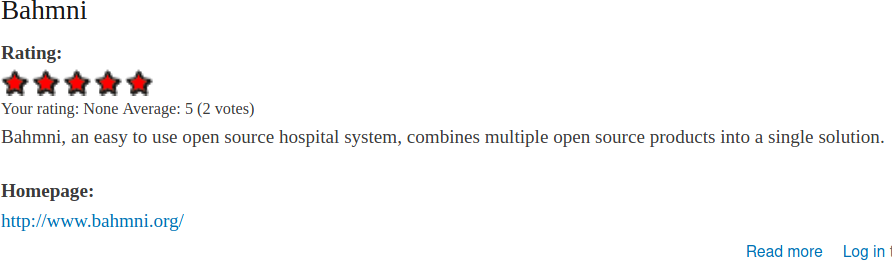
\includegraphics[width=\textwidth]{img/medfloss-bahmni.png}
\end{frame}

\begin{frame}{Medfloss Bahmni Link}
  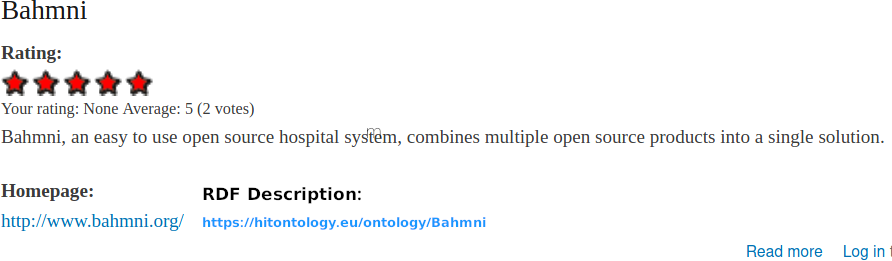
\includegraphics[width=\textwidth]{img/medfloss-bahmni-link.png}
\end{frame}

\begin{frame}{HITO Lifecycle}
  \centering
  \vspace{-0.5cm}
  \includegraphics[height=0.85\textheight]{hitocyclerest.pdf}
\end{frame}


\end{document}
